\documentclass{article}

% Encodings, page setup, paragraph formatting, font
\usepackage[top=0.9in, bottom=1in, left=1.5in, right=1.5in]{geometry}
\usepackage[icelandic]{babel}
\usepackage[T1]{fontenc}
\usepackage[sc]{mathpazo}
\usepackage[parfill]{parskip}
\usepackage{cancel}
% Tables and lists
\usepackage{booktabs,tabularx}
\usepackage{multirow}
\usepackage{enumerate}
\usepackage{adjustbox}
\usepackage{multicol}
\usepackage{enumitem}
\usepackage{xcolor}
% Math
\usepackage{amsmath, amsfonts, amssymb, amsthm}
% Graphics
\usepackage{graphicx}
\usepackage{forest}
\usepackage{tikz}
\usetikzlibrary{positioning, shapes, arrows.meta}
% Custom Commands til að auðvelda lífið
\newcommand{\sv}{\textbf{Svar:}}
\newcommand{\bo}[1]{\textbf{#1}}
\newcommand{\enum}{\begin{enumerate}[label = \alph*.]}


\usepackage{listingsutf8}
\definecolor{commentcolor}{RGB}{255, 0, 255} % Bleikur
\definecolor{keywordcolor}{RGB}{139, 69, 19}   % Brúnn
\definecolor{stringcolor}{RGB}{0, 0, 255}      % Blár
\definecolor{numbercolor}{RGB}{0, 128, 0}      % Grænn
\definecolor{identifiercolor}{RGB}{0, 0, 255}
%Morpho
\lstdefinelanguage{CustomLang}{
    alsoletter={=},
    keywords={rec, fun, if, else, return},
    sensitive=true,
    comment=[l]{;;;},
    commentstyle=\color{commentcolor},
    morestring=[b]",
    stringstyle=\color{stringcolor},
}

\lstset{
    language=CustomLang,
    basicstyle=\ttfamily,
    keywordstyle=\color{keywordcolor},
    commentstyle=\color{commentcolor},
    identifierstyle=\color{identifiercolor},
    stringstyle=\color{stringcolor},   
    showstringspaces=false,
    numbers=none,
    tabsize=2,
    breaklines=true,
    columns=fullflexible,
    keepspaces=true,
    inputencoding=utf8, 
    extendedchars=true,  
    literate=
        {á}{{\'a}}1
        {ð}{{\dh}}1
        {é}{{\'e}}1
        {í}{{\'i}}1
        {ó}{{\'o}}1
        {ú}{{\'u}}1
        {ý}{{\'y}}1
        {þ}{{\th}}1
        {æ}{{\ae}}1
        {ö}{{\"o}}1
        {Á}{{\'A}}1
        {Ð}{{\DH}}1
        {É}{{\'E}}1
        {Í}{{\'I}}1
        {Ó}{{\'O}}1
        {Ú}{{\'U}}1
        {Ý}{{\'Y}}1
        {Þ}{{\TH}}1
        {Æ}{{\AE}}1
        {Ö}{{\"O}}1,
}


% Hyphenation
\hyphenpenalty=5000
% Page and section numbering
\setcounter{secnumdepth}{-1} 
\pagenumbering{gobble}
\title{Forritunarmál}
\author{Benjamín}
\date{11.27.2024}

\begin{document}

\maketitle

\begin{center}
    \Huge{Lokapróf Forritunarmál 2018, 2019, 2021, 2022,2023}

    \bo{Í þessu samansafni tek ég ekki inn 2020 þar sem það er svo frábrugðið hinum prófunum,
    einnig sleppi ég stundum 2021 þar sem það er einnig frábrugðið og var covid próf}
\end{center}



\newpage

\section{Lokanir}

\bo{Hverjar eftirfarandi fullyrðinga um lokanir eru sannar? Tvö röng
svör gefa núll punkta.}


\enum
\item Lokanir eru til í C.
\item Lokanir eru til í Scheme.
\item Lokanir eru til í CAML.
\item Lokanir eru til í Morpho.
\item Lokanir innihalda fallsbendi.
\item Lokanir eru nauðsynlegar til að skila staðværu falli sem skilagildi
      falls í bálkmótuðum forritunarmálum.
\item Lokanir eru aðeins mögulegar ef vakningarfærslur eru í kös.
\item Lokanir innihalda stýrihlekk
\item Lokanir innihalda tengihlekk.
\item Lokanir innihalda straum.
\item Lokanir eru nauðsynlegar til að senda staðvær föll sem viðföng í bálkmótuðum forritunarmálum.
\item Lokanir má nota til að útfæra strauma í scheme.

\end{enumerate}

\begin{tabularx}{\textwidth}{|X|X|X|X|X|X|X|X|X|X|X|X|}
    \hline
    \bo{a} & \bo{b} & \bo{c} & \bo{d} & \bo{e} & \bo{f} & \bo{g} & \bo{h} & \bo{j} & \bo{k} & \bo{l} & \bo{m} \\ \hline
     & & & & & & & & & & & \\ \hline
\end{tabularx}

\newpage

\bo{Hverjar eftirfarandi fullyrðinga um aðgangshlekki (tengihlekki),
stýrihlekki og lokanir eru sannar? Tvö röng svör gefa núll punkta.}

\enum
\item Aðgangshlekkir eru notaðir í bæði bálkmótuðum og öðrum
forritunarmálum.
\item Stýrihlekkir eru notaðir bæði í bálkmótuðum og öðrum
forritunarmálum
\item Lokanir innihalda aðgangshlekk
\item Lokanir innihalda stýrihlekk og aðgangshlekk.
\item Lokanir innihalda vendivistfang og stýrihlekk.
\item Lokanir innihalda fallsbendi.
\item Lokanir innihalda fallsbendi og aðgangshlekk.
\item aðgangshlekkir eru ekki til í Haskell
\item Lokanir eru ekki til í Scheme
\item Stýrihlekkir eru ekki til í CAML.
\item Lokanir eru ekki til í Morpho.
\item Aðgangshlekkir eru ekki til í Java
\item Lokanir eru aðeins mögulegar ef vakningarfærslur eru í kös
\end{enumerate}

\begin{tabularx}{\textwidth}{|X|X|X|X|X|X|X|X|X|X|X|X|}
    \hline
    \bo{a} & \bo{b} & \bo{c} & \bo{d} & \bo{e} & \bo{f} & \bo{g} & \bo{h} & \bo{j} & \bo{k} & \bo{l} & \bo{m}  \\ \hline
     & & & & & & & & & & &  \\ \hline
\end{tabularx}


\newpage
\section{Vakningarfærsla}

\bo{Vakningarfærsla falls í bálkmótuðu forritunarmáli eins og Scheme
inniheldur sum eftirfarandi atriða. Hver? Tvö röng svör gefa núll
stig}

\enum
\item Staðværar breytur fallsins
\item Bendi á vakningarfærslu fallsins sem kallaði á fallið
\item Bendi á vakningarfærslu fallsins sem inniheldur fallið, textalega
séð, ef eitthvert er
\item Skráakerfi tölvunnar
\item Viðföng fallsins
\item Aðgangshlekk (tengihlekk)
\item Stýrihlekk
\item Vendivistfang.
\item Benda á öll föll sem hægt er að kalla á úr fallinu
\item Benda á allar lifandi vakningarfærslur
\item Alla hluti sem til eru í kerfinu.
\item Vakningarfærslur allra falla sem hægt er að kalla á
\item Nöfn allra falla sem hægt er að kalla á
\item Lokun sem vísar á fallið.
\end{enumerate}


\begin{tabularx}{\textwidth}{|X|X|X|X|X|X|X|X|X|X|X|X|X|}
    \hline
    \bo{a} & \bo{b} & \bo{c} & \bo{d} & \bo{e} & \bo{f} & \bo{g} & \bo{h} & \bo{j} & \bo{k} & \bo{l} & \bo{m} & \bo{n} \\ \hline
     & & & & & & & & & & & & \\ \hline
\end{tabularx}

\newpage

\section{Foldun}

Íhugið mydnina sem sýnir földun A,B,C,D og E

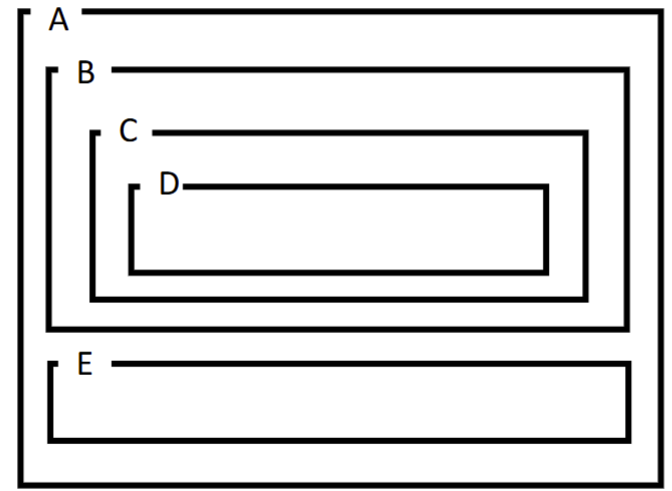
\includegraphics[scale = 1 ]{myndir/AbcdFoldun.png}

Samsvarandi Scheme forritstexti er einnig sýndur í tveimur
jafngildum útgáfum hlið við hlið.

\begin{verbatim}
    (define (A ...)              (define (A ...)
     (define (B ...)              (define (E ...)
      (define (C ...)               ...[stofn E/body of E]
       (define (D ...)            )
        ...[stofn D/body of D]    (define (B ...)
       )                           (define (C ...)
       ...[stofn C/body of C]       (define (D ...)
      )                                ...[stofn D/body of D]
      ...[stofn B/body of B]        )
     )                              ...[stofn C/body of C]
     (define (E ...)               ) 
       ...[stofn E/body of E]      ...[stofn B/body of B]
     )                            )
     ...[stofn A/body of A]       ...[stofn A/body of A]
    )                            )
\end{verbatim}

Fyllið út eftirfarandi töflur með því að setja krossa við sannar fullyrðingar.
Eitt rangt svar gefur núll í einkunn fyrir dæmið.

kalla má A úr:


\begin{tabularx}{\textwidth}{|X|X|X|X|X|}
    \hline
    \bo{A} & \bo{B} & \bo{C} & \bo{D} & \bo{E}\\ \hline
    & & & & \\ \hline
\end{tabularx}

\newpage
Kalla má B úr:


\begin{tabularx}{\textwidth}{|X|X|X|X|X|}
    \hline
    \bo{A} & \bo{B} & \bo{C} & \bo{D} & \bo{E}\\ \hline
    & & & & \\ \hline
\end{tabularx}


\vspace{1cm}

Kalla má C úr:


\begin{tabularx}{\textwidth}{|X|X|X|X|X|}
    \hline
    \bo{A} & \bo{B} & \bo{C} & \bo{D} & \bo{E}\\ \hline
    & & & & \\ \hline
\end{tabularx}

\vspace{1cm}

Kalla má D úr: 


\begin{tabularx}{\textwidth}{|X|X|X|X|X|}
    \hline
    \bo{A} & \bo{B} & \bo{C} & \bo{D} & \bo{E}\\ \hline
    & & & & \\ \hline
\end{tabularx}


\vspace{1cm}

Kalla má E úr:


\begin{tabularx}{\textwidth}{|X|X|X|X|X|}
    \hline
    \bo{A} & \bo{B} & \bo{C} & \bo{D} & \bo{E}\\ \hline
    & & & & \\ \hline
\end{tabularx}

\vspace{1cm}

Staðværar breytur í A má nota í:


\begin{tabularx}{\textwidth}{|X|X|X|X|X|}
    \hline
    \bo{A} & \bo{B} & \bo{C} & \bo{D} & \bo{E}\\ \hline
    & & & & \\ \hline
\end{tabularx}

\vspace{1cm}

Staðværar breytur í B má nota í:


\begin{tabularx}{\textwidth}{|X|X|X|X|X|}
    \hline
    \bo{A} & \bo{B} & \bo{C} & \bo{D} & \bo{E}\\ \hline
    & & & & \\ \hline
\end{tabularx}

\vspace{1cm}

Staðværar breytur í C má nota í:


\begin{tabularx}{\textwidth}{|X|X|X|X|X|}
    \hline
    \bo{A} & \bo{B} & \bo{C} & \bo{D} & \bo{E}\\ \hline
    & & & & \\ \hline
\end{tabularx}

\vspace{1cm}

Staðværar breytur í D má nota í:


\begin{tabularx}{\textwidth}{|X|X|X|X|X|}
    \hline
    \bo{A} & \bo{B} & \bo{C} & \bo{D} & \bo{E}\\ \hline
    & & & & \\ \hline
\end{tabularx}

\vspace{1cm}

Staðværar breytur í E má nota í:


\begin{tabularx}{\textwidth}{|X|X|X|X|X|}
    \hline
    \bo{A} & \bo{B} & \bo{C} & \bo{D} & \bo{E}\\ \hline
    & & & & \\ \hline
\end{tabularx}


\newpage
\section{eitthver forritstexti}
Eftirfarandi forritstexti er í einhverju ímynduðu forritunarmáli.

\begin{verbatim}
    void f(x,y)
    {
        y = 3;
        print x,y;
        x = 2;
    }
    int i,a[10];
    for( i=0 ; i!=10 ; i++ ) a[i]=i+1;
    f(a[a[0]],a[0]);
    print a[0], a[1], a[2], a[3];
\end{verbatim}
Hvað skrifar þetta forrit (sex gildi í hvert skipti) ef viðföngin eru:

\enum
\item \bo{Gildisviðföng }
\item \bo{Tilvísunarviðföng }
\item \bo{Nafnviðföng}
\end{enumerate}

\newpage
\section{Hluti II – Listavinnsla o.fl.}

\bo{spurning 5 möguleikar}
\begin{enumerate}
    \item Skrifið fall í Scheme, CAML, Morpho eða Haskell sem tekur eitt
    viðfang sem er listi lista af fleytitölum milli 0 og 1 og skilar tölu
    sem er stærsta lággildi innri listanna, þ.e. stærst af þeim tölum
    sem fást þegar fundin er minnsta tala í hverjum innri lista. Þið
    skuluð reikna með því að hágildi í tóma menginu sé 0 og lággildi
    í tóma menginu sé 1. Munið fallslýsingar, eins og alltaf. Fallið
    þarf að skila viðeigandi gildi bæði fyrir tóman lista og fyrir lista
    sem einungis inniheldur tóma lista.

    \item Skrifið halaendurkvæmt fall í Scheme, CAML, Morpho eða Haskell,
    sem tekur lista talna $x1, \ldots , xn$ sem viðfang og skilar summunni
    $\sum_{i=1}^{n}X_i^2$. Þið munið þurfa hjálparfall og munið að skrifa réttar
    notkunarlýsingar. Einungis má nota einföld innbyggð föll svo sem
    +, *, null? car, cdr og cons, en ekki flóknari föll svo sem foldl eða
    map.

\end{enumerate}

\bo{spurning 6  möguleikar}
\begin{enumerate}
    \item Skrifið fall zip2 í Scheme, CAML, Morpho eða Haskell sem tekur
    tvíundaraðgerð (fall) og tvo jafnlanga lista sem viðföng og skilar
    lista þeirra útkomna sem fást þegar tvíundaraðgerðinni er beitt á
    gildin í listunum, par fyrir par. Til dæmis, í Scheme þá ætti
    segðin (zip2 + ‘(1 2 3) ‘(4 5 6)) að skila listanum (5 7 9). Notið
    einungis einfaldar aðgerðir svo sem car, cdr, cons, null?

    \item Skrifið halaendurkæmt fall zipMapRev í Scheme, CAML,
    Morpho eða Haskell sem tekur tvö viðföng sem eru jafnlangir
    listar. Fyrra viðfangið skal vera listi einundarfalla, 𝑓1, ... , 𝑓𝑛, og
    seinna viðfangið skal vera listi gilda 𝑥1, ... , 𝑥𝑛 þannig að sérhvert
    𝑥𝑖 er löglegt viðfang í samsvarandi 𝑓𝑖. Fallið skal skila
    viðsnúnum lista gildanna sem föllin skila þegar þeim er beitt á
    gildin, þ.e. lista með gildunum 𝑓𝑛(𝑥𝑛), ... , 𝑓1(𝑥1), í þeirri röð. Notið
    einungis einfaldar aðgerðir svo sem car, cdr, cons, null?. Í
    Morpho má nota lykkju, með fastarðingu lykkju
\end{enumerate}

\bo{spurning 7 möguleikar}
\begin{enumerate}
    \item Skrifið ykkar eigin útgáfur af föllunum tveimur sem í CAML Light
    eru kölluð it_list og list_it. Í Haskell eru þau kölluð foldl og foldr. Þið
    megið skrifa þessi föll í Scheme, CAML, Morpho eða Haskell. Notið
    ekki lykkjur í Morpho. Kallið föllin myLeft og myRight. Þið megið
    nota aðra röð viðfanga en í it_list og list_it. Sjáið til þess að a.m.k.
    annað fallið sé halaendurkvæmt og tiltakið hvort það er. Notið
    aðeins einföld innbyggð föll svo sem car, cdr og null?.

    \item Skrifið tvö föll, findFirst og findLast í Scheme, CAML, Morpho
    eða Haskell, sem bæði taka eitt viðfang sem skal vera listi
    heiltalna. Skilagildið úr findFirst skal vera lengsti undirlisti
    viðfangsins sem hefur null í hausnum. Ef ekkert núll er í
    viðfanginu skal skila tómum lista. Skilagildið úr findLast skal
    vera stysti undirlisti viðfangsins sem hefur null í hausnum. Ef
    viðfangið inniheldur ekkert null skal skila tómum lista. Í þessu
    dæmi reiknum við með að undirlisti lista sé listi sem fenginn er
    með því að fjarlægja hausinn null sinnum eða oftar
\end{enumerate}


\end{document}